\documentclass[english, version-2020-11]{uzl-thesis}
\UzLStyle{computer modern oldschool design}
\usepackage{comment}
\usepackage{float}

\UzLThesisSetup{
Masterarbeit,
Verfasst              = {am}{Institut für Technische Informatik},
Titel auf Deutsch     = {
    Bewertung von RISC-V-Enklaven: Leistungsbenchmarks und bewährte Konfigurationspraktiken
}, 
Titel auf Englisch    = {
    Evaluating RISC-V Enclaves: Performance Benchmarks and Configuration Best Practices 
},
Autor                 = {Basil Ugbomoiko},
Betreuerin            = {Dr.-Ing. Saleh Mulhem},
Mit Unterstützung von = {Henrik Strunck, M.Sc},
Studiengang           = {IT Security},
Datum                 = {31. August 2025},
Abstract = {This thesis evaluates the performance of Keystone enclaves, an open-source Trusted Execution Environment (TEE) designed for RISC-V platforms. Keystone enables secure computation by isolating sensitive workloads from the rest of the system. To assess its performance, the study benchmarks critical system parameters, including the number of CPU cores, cache size, memory allocation, and enclave configuration. Using industry-standard benchmarking tools such as Dhrystone and CoreMark, the research measures execution time, context switch overhead, memory latency, and CPU utilization across a range of hardware and software configurations. The experimental analysis identifies key performance bottlenecks that impact the efficiency of enclave execution. Based on these findings, the study presents configuration best practices and tuning recommendations tailored to various workload profiles, such as compute-bound, memory-intensive, and mixed applications. The insights gained from this evaluation contribute to optimizing the deployment of Keystone enclaves, making them more viable for real-world use cases that demand secure and efficient execution on RISC-V architectures.},
Zusammenfassung = {Diese Arbeit bewertet die Leistung von Keystone-Enklaven, einer Open-Source Trusted Execution Environment (TEE) für RISC-V-Plattformen. Keystone ermöglicht sichere Berechnungen, indem sensible Workloads vom restlichen System isoliert werden. Zur Leistungsbewertung werden zentrale Systemparameter wie die Anzahl der CPU-Kerne, die Cache-Größe, die Speicherzuweisung und die Konfiguration der Enklave untersucht. Mithilfe standardisierter Benchmarking-Tools wie Dhrystone und CoreMark werden Ausführungszeit, Kontextwechsel-Overhead, Speicherlatenz und CPU-Auslastung unter verschiedenen Hardware- und Softwarekonfigurationen gemessen. Die experimentelle Analyse identifiziert wichtige Leistungsengpässe, die die Effizienz der Enklaven beeinträchtigen. Auf Basis dieser Erkenntnisse werden Konfigurationsrichtlinien und Optimierungsempfehlungen vorgestellt, die auf unterschiedliche Workload-Profile zugeschnitten sind, z. B. rechenintensive, speicherintensive und gemischte Anwendungen. Die gewonnenen Erkenntnisse tragen dazu bei, den Einsatz von Keystone-Enklaven zu optimieren und ihre praktische Anwendbarkeit in sicherheitskritischen Bereichen auf RISC-V-Architekturen zu verbessern.},
Numerische Bibliographie
} % Put your \UzLStyle and \UzLThesisSetup here

\begin{document}

\chapter{Introduction}

Modern computing increasingly relies on platforms that operate in potentially untrusted environments. These include public cloud infrastructures, multi-tenant servers, and distributed edge devices, where sensitive data and critical computations may be exposed to compromised software stacks or malicious actors. In such contexts, ensuring the confidentiality and integrity of both data and execution is a fundamental requirement. Conventional security mechanisms, such as access control and encryption, are often insufficient in scenarios where the underlying operating system, hypervisor, or even firmware may be compromised.

To address these challenges, Trusted Execution Environments (TEEs) have emerged as a compelling solution. TEEs provide hardware-assisted isolation mechanisms that enable the execution of code in a protected context, referred to as an enclave. This enclave is designed to be resilient to attacks originating from untrusted system components, including the operating system and other user-space applications. By establishing a secure boundary around sensitive code and data, TEEs allow developers to implement trustworthy services even on compromised hosts.

Several commercial implementations of TEEs exist today, with Intel Software Guard Extensions (SGX) and ARM TrustZone being the most prominent examples. These technologies have demonstrated the practical viability of hardware-enforced isolation, and they have been integrated into a variety of real-world applications, from digital rights management to secure machine learning inference. However, despite their utility, these solutions are inherently proprietary and closed-source. This lack of transparency imposes significant constraints on researchers, developers, and system architects who wish to investigate alternative TEE designs, customize security mechanisms, or perform formal verification. Moreover, the architectural rigidity of these platforms limits their adaptability to emerging use cases, especially in academic or experimental contexts.

To overcome these limitations, the Keystone framework introduces an open-source, modular TEE architecture built atop the RISC-V instruction set architecture (ISA). RISC-V itself is an open, extensible ISA that has gained significant traction in both academic and industrial settings. Keystone leverages RISC-V's flexibility to enable fine-grained control over enclave behavior and to support a minimal, verifiable trusted computing base (TCB). The framework allows researchers and developers to explore custom enclave policies, experiment with hardware-software co-design, and perform reproducible evaluations in a controlled setting.

This thesis presents a detailed investigation into the Keystone TEE framework. It explores Keystone's architectural foundations, its use of RISC-V hardware features such as Physical Memory Protection (PMP), and its support for dynamic enclave management. Special attention is paid to the performance implications of enclave isolation, as measured through controlled benchmarking in a virtualized environment. By evaluating Keystone under varying execution conditions, this work seeks to provide a rigorous assessment of its efficiency and suitability for secure computation on emerging RISC-V platforms.
\chapter{Introduction}
\label{chap:intro}

In the rapidly evolving landscape of modern computing, an undeniable shift has taken place over the past decade. Computing no longer happens exclusively within the safe confines of dedicated, physically secured machines operated by trusted personnel. Instead, it is increasingly conducted across a wide array of environments that range from large-scale, multi-tenant cloud platforms to geographically dispersed edge devices deployed in untrusted, sometimes hostile, settings. These emerging scenarios offer unparalleled scalability, accessibility, and flexibility but simultaneously pose profound new challenges to the foundational assumptions upon which traditional system security models have long been based.

Consider, for example, a cloud computing environment where organizations lease computational resources from a third-party provider. While this model delivers significant economic and operational advantages, it necessarily requires placing sensitive data and critical computations on infrastructure controlled, at least in part, by entities outside the organization’s direct control. In such environments, the software stack—from firmware and bootloaders to the operating system and hypervisor—may be susceptible to compromise through vulnerabilities, misconfigurations, or even insider threats. Similarly, edge devices deployed in remote locations may operate without continuous physical supervision, making them vulnerable to physical tampering or software-based attacks. In all these cases, the question arises: how can one guarantee that sensitive computations execute correctly and confidentially, even when the underlying platform may be compromised or untrusted?

Traditional security approaches, such as enforcing access controls, employing encryption for data at rest or in transit, or leveraging virtualization-based isolation, offer important protections but are often insufficient in these adversarial contexts. These mechanisms fundamentally rely on the integrity of the underlying system software to enforce security policies. Once that trust is broken—for example, if a privileged kernel or hypervisor is subverted—malicious actors may gain unauthorized access to secrets, manipulate computations, or subvert the system’s intended behavior. As a result, there has been a growing recognition of the need for a fundamentally different approach: one that can provide strong guarantees about the confidentiality and integrity of code and data, even in the face of potentially compromised system components.

This pressing need has catalyzed the development of Trusted Execution Environments (TEEs), a class of hardware-assisted security mechanisms designed to establish a secure and isolated environment within an untrusted platform. A TEE creates a trusted “enclave” or protected region of execution where sensitive code and data reside, shielded from the rest of the system, including the operating system, hypervisor, and other software running on the host. By leveraging hardware features that enforce strict isolation and memory protection boundaries, TEEs aim to provide a sanctuary of trust—a secure vault in which computations can proceed without fear of interference or observation by unauthorized parties.

The promise of TEEs is compelling: they enable the secure execution of sensitive workloads such as cryptographic key management, digital rights enforcement, confidential cloud computing, and privacy-preserving data analytics. Over the past several years, commercial implementations have emerged, most notably Intel’s Software Guard Extensions (SGX) and ARM’s TrustZone technology, each offering unique approaches to enclave creation and hardware isolation. Intel SGX, for example, introduces user-space enclaves with hardware-enforced memory encryption and attestation capabilities, allowing remote verification of enclave authenticity. ARM TrustZone takes a different approach, partitioning the processor into Secure and Normal worlds to separate trusted code from the rest of the system.

Despite their successes and practical deployments, these commercial TEEs come with a number of significant limitations that hinder their applicability in research, experimental settings, and use cases requiring flexibility and transparency. Both SGX and TrustZone are proprietary technologies with closed-source implementations, limiting independent analysis, verification, and modification. Their architectural designs are relatively rigid, optimized for particular use cases, and do not easily accommodate novel security policies, alternative enclave management strategies, or supervisor-mode enclave execution. Moreover, their Trusted Computing Bases (TCBs) can be substantial, complicating efforts at formal verification and security assurance. These challenges collectively motivate the exploration of open, extensible TEE architectures that can empower researchers and practitioners to experiment, customize, and extend trusted execution mechanisms without the constraints imposed by proprietary solutions.

It is within this context that the Keystone framework has emerged as a pioneering open-source TEE architecture built atop the RISC-V instruction set architecture (ISA). RISC-V, an open and extensible ISA, has attracted substantial attention in academia and industry alike for its flexibility, simplicity, and openness. Keystone leverages these advantages to provide a modular, fully open TEE framework that supports fine-grained control over enclave behavior and a minimal trusted computing base. Notably, Keystone harnesses RISC-V’s hardware capabilities such as Physical Memory Protection (PMP) to implement hardware-enforced isolation, enabling dynamic enclave management and runtime configurability rarely available in existing TEEs.

Keystone’s open design philosophy not only facilitates deep architectural exploration and formal verification but also enables the development of novel security primitives and policies tailored to emerging application domains. Its modularity supports supervisor-level enclave components, dynamic loading, and interaction with Linux-based host environments, making it well-suited for research, prototyping, and education. However, the flexibility offered by Keystone comes with inherent challenges. For instance, RISC-V’s PMP architecture, while powerful, imposes a limited number of protection entries, constraining the number of concurrent enclaves and complicating memory management. Additionally, the performance overhead induced by enclave isolation—especially when executing memory-intensive or computationally demanding workloads such as post-quantum cryptographic algorithms—necessitates thorough empirical evaluation to guide practical deployment and future hardware design.

This thesis undertakes a comprehensive investigation of the Keystone framework, focusing on its architectural foundations, practical deployment in a fully virtualized RISC-V environment, and performance characteristics under representative workloads. Through methodical benchmarking using standard synthetic tests and cryptographic workloads, this work illuminates the complex trade-offs between security, performance, and scalability inherent to Keystone’s design. The study further documents the intricacies of configuring and debugging Keystone enclaves in an emulator, addressing the challenges posed by hardware constraints such as PMP entry exhaustion. By providing a rigorous empirical characterization of Keystone’s runtime behavior and scalability limits, this thesis contributes valuable insights to the open TEE community and lays the groundwork for future enhancements in RISC-V based secure execution environments.

In the following sections, this introduction will first articulate the specific contributions of this thesis in detail. It will then situate this work within the broader context of related research and commercial TEE developments. Finally, an overview of the thesis structure will guide the reader through the chapters that follow, setting the stage for an in-depth exploration of Keystone and its capabilities.

\section{Contributions of this Thesis}

This thesis makes several key contributions that advance the understanding and evaluation of Trusted Execution Environments, particularly focusing on the open-source Keystone framework and its RISC-V hardware foundation.

\begin{itemize}
    \item \textbf{Comprehensive Architectural Analysis:} A detailed exposition of Keystone’s design is presented, highlighting its Security Monitor (SM), enclave runtime, and user-level application interactions. This includes an exploration of how RISC-V’s privilege levels and Physical Memory Protection (PMP) mechanisms are employed to establish and enforce robust isolation boundaries between enclaves and untrusted system components.
    
    \item \textbf{Comparative Evaluation with Commercial TEEs:} The thesis performs a thorough comparative study positioning Keystone alongside Intel SGX and ARM TrustZone. This analysis elucidates key architectural distinctions, including enclave lifecycle management, privilege separation, Trusted Computing Base size, scalability, and extensibility. This contextualization highlights Keystone’s unique advantages in openness, modularity, and adaptability for research and experimentation.
    
    \item \textbf{Virtualized Deployment and Toolchain Documentation:} A fully virtualized deployment of Keystone is demonstrated using a RISC-V-specific QEMU emulator. This approach allows experimentation independent of physical hardware availability. The thesis provides detailed documentation of the build environment, toolchain configuration, emulator setup, and debugging workflows, establishing a reproducible methodology for future work.
    
    \item \textbf{Empirical Performance Evaluation:} Using established benchmarks such as Dhrystone and CoreMark, alongside a computationally demanding post-quantum cryptographic workload (Kyber), the thesis quantifies runtime overheads incurred by enclave isolation. It explores how varying system parameters—such as CPU core count, memory allocation, and cache sizes—affect enclave performance and stability.
    
    \item \textbf{Analysis of Hardware-Induced Scalability Constraints:} The limited number of PMP entries and its impact on enclave concurrency and lifecycle management is carefully analyzed. The thesis identifies bottlenecks and proposes strategies to mitigate the effects of PMP exhaustion on system scalability and enclave deployment.
    
    \item \textbf{Identification and Documentation of Runtime Failure Modes:} Through extensive testing, the thesis uncovers failure scenarios arising from PMP limitations and enclave memory protection policies, contributing practical insights and guidance to the Keystone community for improving robustness and fault tolerance.
\end{itemize}

\section{Related Work}

Trusted Execution Environments (TEEs) have become a cornerstone for securing computation on untrusted platforms by isolating sensitive code and data from the rest of the system. The landscape of TEE technologies includes Intel SGX, ARM TrustZone, AMD SEV, and emerging open-source frameworks like Keystone, each offering distinct security guarantees, performance trade-offs, and hardware dependencies.

Intel SGX~\cite{akkram2020scientific, kumar2022sgxgauge} provides strong confidentiality and integrity guarantees via isolated enclaves backed by hardware-enforced memory encryption. However, SGX suffers from limited enclave page cache (EPC) size, causing significant performance degradation when working sets exceed EPC limits, as observed by Kumar et al.~\cite{kumar2022sgxgauge}. Moreover, the overheads in enclave transitions and paging have been documented in multiple studies~\cite{akkram2020scientific, krahn2020teemon}.

ARM TrustZone~\cite{suzaki2021tsperf} takes a different approach by partitioning the processor into secure and normal worlds, enabling lightweight isolation for Trusted Applications but with generally weaker isolation guarantees than SGX. Its performance impact tends to be lower, yet TrustZone’s capabilities and APIs are less standardized, which complicates broad adoption and benchmarking~\cite{turn0search9}.

AMD SEV and newer technologies such as SEV-SNP offer memory encryption and integrity protections for virtual machines, providing scalable enclave-like isolation for cloud workloads. Coppolino et al.~\cite{coppolino2025experimental} experimentally evaluated SEV and TDX against SGX, revealing performance and transparency trade-offs that influence their suitability for different application scenarios.

In parallel, open-source efforts like Keystone~\cite{Lee2019} aim to democratize TEE development by providing a modular framework on RISC-V processors, supporting flexible enclave configurations and custom security policies. Research into Keystone’s memory models and sharing mechanisms~\cite{yu2022elasticlave, lee2022cerberus} has demonstrated improved performance and formally verified security properties, addressing common TEE bottlenecks such as enclave memory management overhead.

Benchmarking and performance measurement frameworks are crucial to evaluate these TEEs fairly and holistically. TS-perf~\cite{suzaki2021tsperf} offers a unified performance suite targeting multiple TEE architectures, including SGX, TrustZone, and Keystone, facilitating comparative studies. Other benchmarking efforts include SGXGauge~\cite{kumar2022sgxgauge}, which specifically assesses Intel SGX overheads under different workload characteristics, and traditional CPU benchmarks like Dhrystone~\cite{weiss2002dhrystone, york2002benchmarking} and CoreMark~\cite{gal2012exploring}, adapted for enclave contexts.

Continuous monitoring tools like TEEMon~\cite{krahn2020teemon} help identify runtime bottlenecks by tracking enclave performance metrics with modest overheads, enabling dynamic optimization and debugging.

Recent surveys~\cite{Survey2023, turn0search5} provide comprehensive overviews of TEE design choices, common pitfalls, and application domains, highlighting the need for standardized performance evaluations and security validations.

While the state of the art has advanced significantly, challenges remain in balancing security, performance, and programmability across diverse hardware platforms and threat models. This work builds on these prior efforts by focusing on comprehensive performance evaluation across multiple TEEs using realistic workloads, emphasizing the modularity and transparency advantages offered by Keystone and comparing them with established commercial solutions.

\section{Structure of this Thesis}

This thesis is structured to progressively build the reader’s understanding of Trusted Execution Environments, with an emphasis on the Keystone framework and its RISC-V underpinnings. Each chapter deepens the narrative from foundational concepts to practical experimentation and critical analysis.

\begin{itemize}
    \item \textbf{Chapter~\ref{chap:intro}} lays the groundwork by introducing the motivation for secure computing in untrusted environments, detailing the contributions of this work, surveying relevant literature, and providing an overview of the thesis structure.
    
    \item \textbf{Chapter~\ref{chap:background}} presents essential background material on Trusted Execution Environments, the Keystone framework, and RISC-V architectural features such as Physical Memory Protection. It also introduces the Kyber post-quantum key encapsulation mechanism used as a cryptographic benchmark.
    
    \item \textbf{Chapter~\ref{chap:methodology}} describes the experimental setup, including the virtualized RISC-V testbed, benchmark selection criteria, parameter tuning, and measurement methodologies ensuring rigor and reproducibility.
    
    \item \textbf{Chapter~\ref{chap:benchmarking}} reports detailed empirical results exploring the performance impact of enclave isolation under different system configurations and workloads, identifying key overheads and architectural bottlenecks.
    
    \item \textbf{Chapter~\ref{chap:discussion}} synthesizes findings from prior chapters to discuss the trade-offs inherent in enclave design and execution, highlighting implications for future hardware and software secure computing architectures.
    
    \item \textbf{Chapter~\ref{chap:conclusion}} concludes the thesis by summarizing main contributions, reflecting on their broader significance, and outlining promising avenues for further research, including hardware extensions and formal verification approaches.
\end{itemize}


\chapter{Background and System Architecture}
The Keystone framework is built on the RISC-V instruction set architecture, which provides a unique foundation for secure system design due to its open specification and modular extensibility. Unlike traditional ISAs that are controlled by single vendors, RISC-V encourages community-driven enhancements and supports custom extensions, making it particularly attractive for trusted computing research and development. Its clean and well-documented privilege model allows for the implementation of isolation mechanisms that are critical to the construction of TEEs.

RISC-V defines three primary privilege levels: user mode (U-mode), supervisor mode (S-mode), and machine mode (M-mode). These privilege levels are hierarchical, with M-mode having the highest authority over system resources. M-mode has direct access to all hardware features and is responsible for critical functions such as interrupt control, exception handling, and access to physical memory protection mechanisms. Keystone leverages this privilege model by placing its Security Monitor (SM)—the core of the TCB—in M-mode. The SM is responsible for managing enclaves, enforcing memory isolation, and mediating access to sensitive system operations. By situating the TCB in M-mode, Keystone ensures that enclave isolation policies are enforced at the highest level of privilege, thereby minimizing the attack surface.

A central hardware feature used by Keystone is Physical Memory Protection (PMP), introduced in version 1.10 of the RISC-V Privilege Specification. PMP enables M-mode software to define access permissions for specific physical memory regions, controlling which lower-privilege modes (U and S) may read, write, or execute code in those regions. This capability forms the basis of Keystone’s memory isolation model. Each enclave is allocated a private memory region protected by PMP, ensuring that neither the host operating system nor any unauthorized software can access its contents. PMP rules are enforced directly by hardware, providing strong guarantees of isolation that are resistant to software-based attacks.

In addition to memory protection, RISC-V supports a flexible trap and exception handling mechanism. M-mode can intercept and handle all traps, but may delegate certain classes of exceptions—such as system calls and page faults—to S-mode for performance optimization. This delegation allows the enclave runtime to cooperate with the host operating system for memory management tasks, while still maintaining strict control over enclave boundaries. The virtual memory subsystem is managed through the standard RISC-V MMU, which translates virtual addresses to physical addresses using multi-level page tables. Keystone leverages this infrastructure to support enclaves that operate with their own private address spaces, protected by PMP from tampering or inspection.

Importantly, the use of standard programming models and toolchains for M-mode software development makes the Keystone Security Monitor both maintainable and extensible. Unlike microcode or hardwired logic, which are difficult to audit and update, the SM is implemented in C and can be subjected to conventional testing and formal verification techniques. This increases the transparency and trustworthiness of the TCB, which is a critical requirement for secure system design.

Taken together, the combination of RISC-V’s privilege hierarchy, PMP, trap delegation mechanisms, and extensibility provides a solid foundation for implementing robust and configurable TEEs. The Keystone framework capitalizes on these features to deliver a flexible and open platform for secure enclave execution, while remaining faithful to the RISC-V philosophy of openness and modularity.

\section{Trusted Execution Environments}
Trusted Execution Environments (TEEs) are isolated computing environments that provide strong security guarantees for code and data execution, even in the presence of potentially compromised operating systems and applications. They achieve this by leveraging hardware-based isolation mechanisms to establish secure boundaries, often called enclaves, where sensitive computation can occur without interference from the rest of the system. TEEs aim to ensure confidentiality and integrity through careful hardware and software co-design, minimizing the trusted computing base (TCB) and mitigating a wide range of software attacks. While several commercial TEEs, such as Intel Software Guard Extensions (SGX) and ARM TrustZone, demonstrate the feasibility and practical relevance of enclave-based secure execution, their closed-source and inflexible designs limit research and hardware/software co-design opportunities. This has motivated the development of open TEE frameworks like Keystone, built on RISC-V—an open and extensible instruction set architecture. A key architectural feature of TEEs is privilege separation, where a minimal TCB executes in a highly privileged mode controlling access to critical physical resources, while the operating system and applications run in less privileged, untrusted modes.

\section{Keystone architecture overview}

Keystone represents an open-source framework designed to facilitate the architecture and implementation of Trusted Execution Environments (TEEs) leveraging hardware enclaves on RISC-V processors. Its primary objective is to enable the construction of customizable TEEs optimized for specific RISC-V platforms, thereby achieving enhanced performance, reduced trusted computing base (TCB) complexity, and improved programmability tailored to distinct workloads and security threat models.

A typical Keystone-capable system architecture comprises multiple components distributed across different privilege modes of the RISC-V privilege hierarchy. The foundational hardware is a trusted CPU package integrating Keystone-compatible RISC-V cores and a silicon root of trust, potentially augmented by features such as cache partitioning, memory encryption, and secure randomness sources. The core security functionality is governed by the Security Monitor (SM), a minimalistic M-mode software component embodying the system's TCB. The SM is responsible for enclave lifecycle management and enforces isolation boundaries between enclaves and the untrusted operating system (OS).

Keystone’s Security Monitor (SM), executing at the highest privilege level (M-mode), serves as the linchpin of the system’s trusted computing base. Beyond enclave lifecycle management, the SM enforces fine-grained memory isolation policies and orchestrates enclave scheduling, maintaining strict control over resource access to prevent unauthorized interference.

\begin{figure}[htbp]
    \centering
    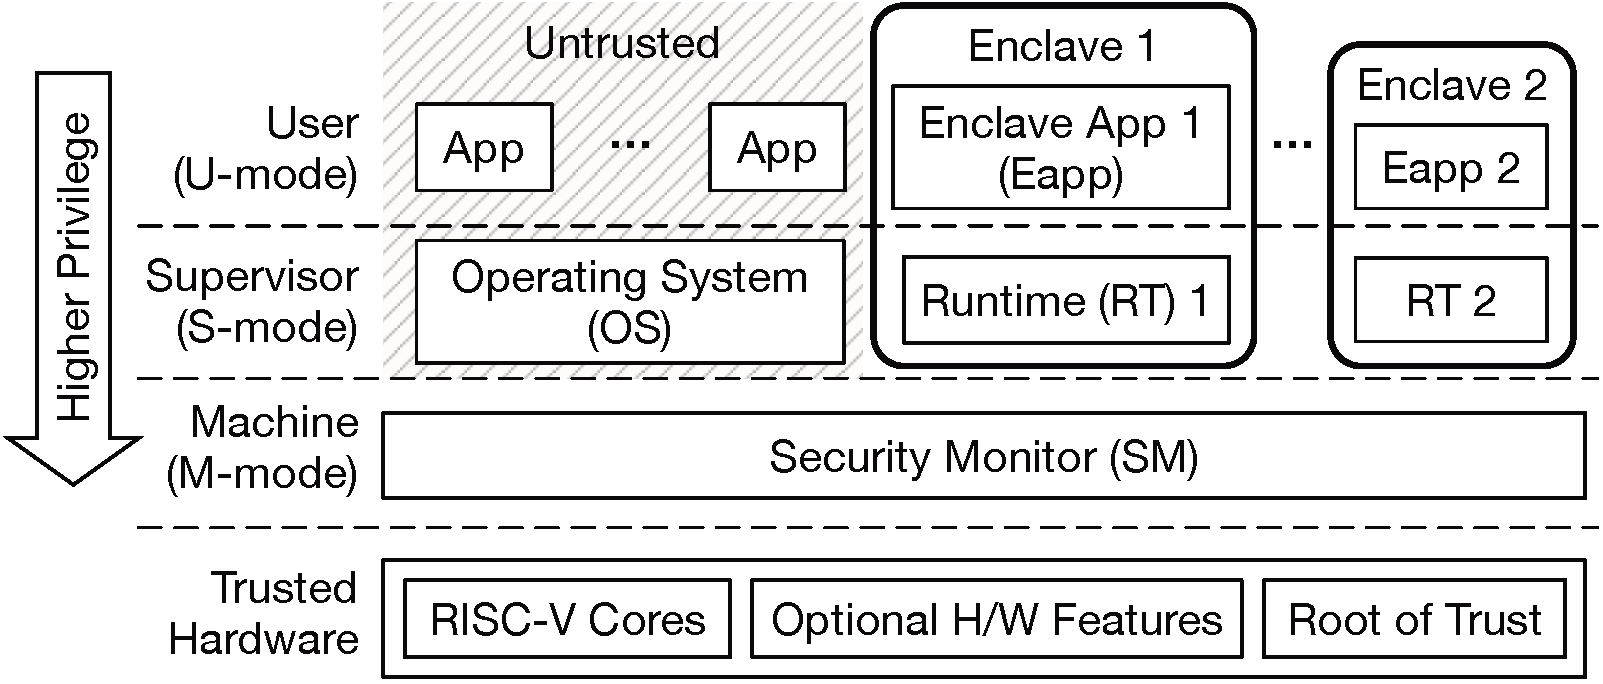
\includegraphics[width=0.9\linewidth]{figures/keystone_overview.png}
    \caption{Overview of the Keystone architecture illustrating components such as the Security Monitor, enclave runtime, and the privilege hierarchy.}
    \label{fig:keystone_overview}
\end{figure}

Enclaves, the fundamental isolation units in Keystone, operate within dedicated physical memory regions inaccessible to the OS and other enclaves. Physical Memory Protection (PMP), a hardware-assisted mechanism controlled by the SM, restricts access to enclave memory exclusively to the enclave and the SM, thus preserving confidentiality and integrity even in the event of OS compromise.

Each enclave comprises two principal layers: the user-level enclave application (eapp) and a supervisor-level runtime environment. The eapp executes user-specific logic within the enclave, while the runtime, operating in supervisor mode (S-mode), manages system calls, exception handling, and virtual memory services intrinsic to enclave operation. This layered design provides a clear separation of concerns, reducing attack surfaces and allowing for customized security policies adapted to workload requirements.

Keystone’s workflow delineates distinct roles for platform providers and enclave developers, fostering modularity and flexibility. Platform providers undertake the compilation and deployment of the SM tailored to the target hardware, ensuring integration of the root of trust and hardware-specific functionalities. Enclave developers leverage the Keystone SDK to construct enclave applications alongside their runtimes and host binaries, which are subsequently packaged and deployed on the target platform independently of underlying hardware specifics.

Furthermore, Keystone supports remote attestation mechanisms, enabling verification of enclave authenticity and integrity prior to provisioning sensitive data or executing critical workloads. This capability is essential for secure deployment in distributed and cloud environments.

The enclave lifecycle progresses through three stages: creation, execution, and destruction. Creation involves the host allocating enclave private memory (EPM), populating it with enclave page tables, runtime, and application binaries, and invoking the SM to isolate the enclave via PMP. During execution, the SM orchestrates transitions into and out of the enclave, dynamically adjusting PMP permissions to maintain strict isolation. Destruction securely clears the enclave’s EPM and reclaims resources, ensuring no residual data remains.

\begin{figure}[htbp]
    \centering
    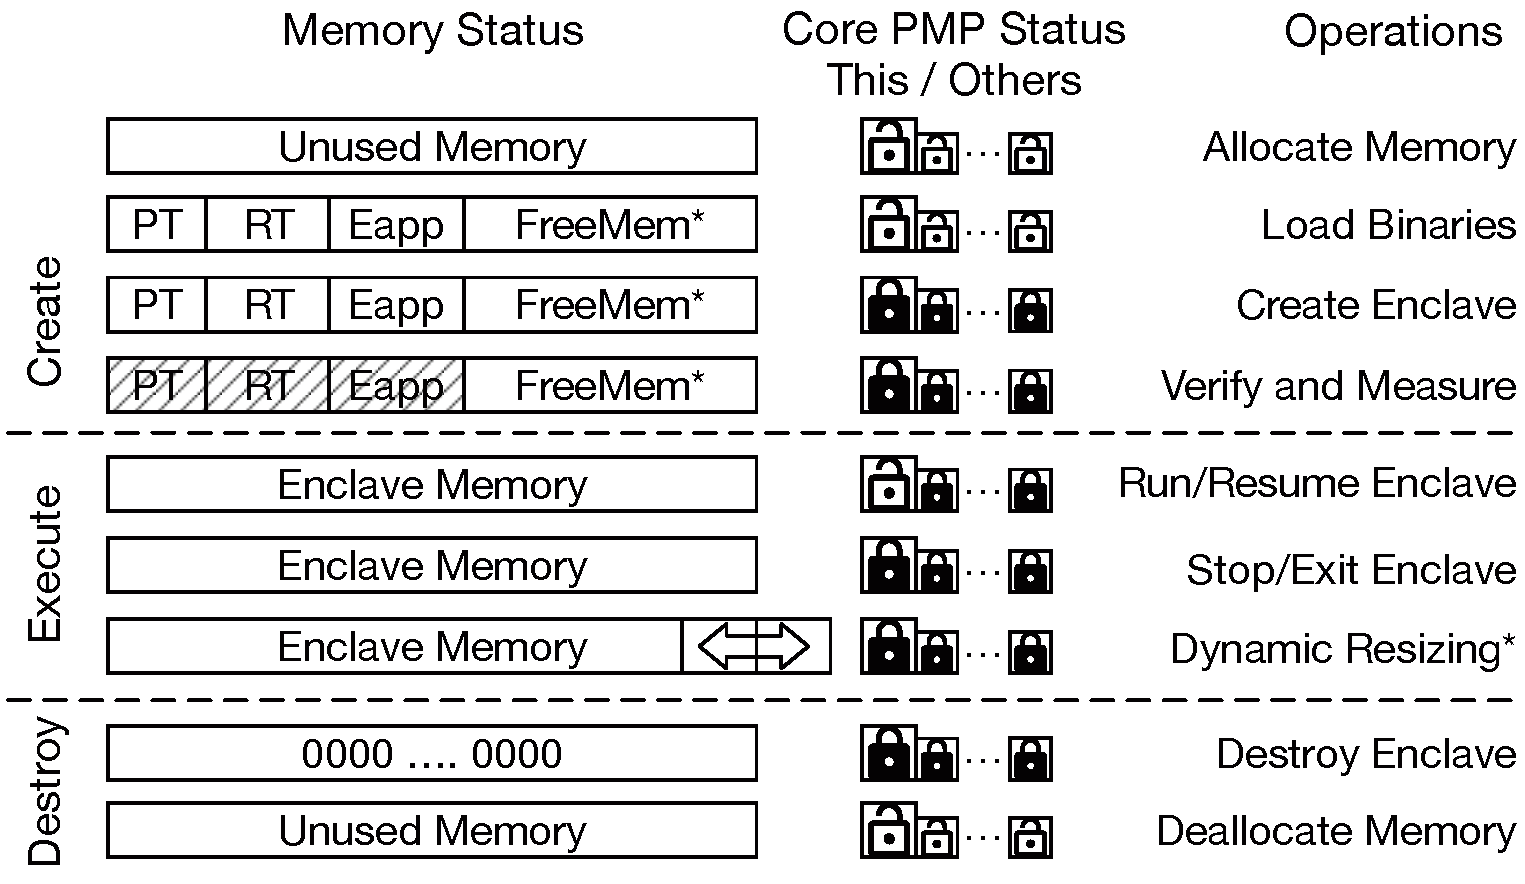
\includegraphics[width=0.9\linewidth]{figures/enclave_lifecycle.png}
    \caption{Stages of a Keystone enclave lifecycle: creation, execution, and destruction.}
    \label{fig:enclave_lifecycle}
\end{figure}

Keystone’s design also facilitates extensibility, allowing for integration of advanced security features such as secure I/O, cryptographic accelerators, and hardware-assisted debugging. This adaptability future-proofs the architecture, enabling continuous evolution of TEE capabilities aligned with emerging threats and diverse application demands on RISC-V platforms.

\section{Comparison with other TEEs}

\section{Performance considerations in TEEs}

\chapter{Methodology}
The primary objective of this thesis is to assess the performance impact of Keystone’s enclave isolation mechanisms on typical embedded and systems-level workloads. Specifically, the study seeks to quantify the computational overhead introduced by executing applications within a Keystone enclave, as compared to their execution in a conventional, non-isolated environment. To achieve this, a series of carefully controlled experiments were designed and executed within a virtualized RISC-V system based on QEMU.

All benchmarks were executed in an emulated environment configured for the RV64GC architecture, which is representative of 64-bit RISC-V systems targeted by Keystone. The use of QEMU for emulation allowed for fine-grained control over the system environment, ensured repeatability, and eliminated the variability introduced by physical hardware, such as thermal throttling or hardware-specific optimizations. Although virtualized, the emulation accurately models instruction execution, privilege transitions, memory access patterns, and I/O behavior, making it suitable for preliminary performance evaluation.

To evaluate the impact of enclave execution, each benchmark was implemented as a standalone enclave application (referred to as an “eapp”), accompanied by a corresponding host application that manages enclave lifecycle events. The host application, running in user space, is responsible for initializing the enclave, loading the benchmark binary, invoking enclave entry points, and handling edge calls used for communication between the enclave and the host. The enclave application, in contrast, is isolated by the Keystone runtime and contains only the benchmark logic and internal data structures. This modular separation ensures that the same benchmark code can be executed both natively (without an enclave) and securely (within an enclave) without structural modification, enabling an accurate comparative analysis.

The evaluation involved executing each benchmark—Dhrystone and CoreMark—under two distinct configurations:

\begin{enumerate}
\item \textit{Native Execution:} The benchmark runs as a conventional user-space process within the QEMU-emulated Linux system, without invoking Keystone enclave services.
\item \textit{Enclave Execution:} The benchmark is loaded into a Keystone enclave, with isolation enforced by the Security Monitor using PMP.
\end{enumerate}

Each benchmark was run multiple times (typically ten iterations per configuration) to account for performance variability and ensure statistical robustness. For each run, metrics such as total execution time, throughput (measured in DMIPS for Dhrystone and iterations per second for CoreMark), and standard deviation were collected. The comparative analysis focused on the relative performance degradation observed in the enclave configuration, thereby providing a direct measurement of the cost of security.

This methodology enables a nuanced understanding of how Keystone’s isolation features influence real-world performance metrics. The controlled nature of the test environment, coupled with repeated measurement and the use of industry-standard benchmarks, ensures that the results are both meaningful and reproducible. By isolating the effect of enclave execution, this study contributes valuable insights into the trade-offs between security and efficiency in open-source TEE architectures.
\section{Experimental setup}
%The experimental setup utilizes the Keystone-enhanced QEMU emulator running on an Ubuntu host operating system. This configuration allows for flexible development and testing of Keystone enclaves in a controlled environment without requiring physical RISC-V hardware. The Ubuntu host provides a stable platform for building and deploying enclave binaries, and it facilitates the integration of the Keystone kernel driver and SDK.

The Keystone framework was evaluated using a RISC-V specific fork of the QEMU emulator on an Ubuntu 22.04 host system. This configuration allowed testing of Keystone enclaves in a controlled virtualized environment, avoiding the need for physical RISC-V hardware. The system was configured to emulate the RV64 architecture for evaluating Keystone’s performance.

The build process for Keystone utilized the Make and Buildroot tools. Key configuration options included the selection of the QEMU virtual platform, the RV64 architecture, and the corresponding Buildroot configuration. Keystone was initiated in the QEMU environment with the following command:

\begin{verbatim}
make run
\end{verbatim}

This command launched the Security Monitor and the Linux OS. Within the QEMU guest, the Keystone kernel driver was manually loaded using:

\begin{verbatim}
modprobe keystone-driver
\end{verbatim}

For debugging, Keystone was run in debug mode with the QEMU GDB server connected to inspect memory protection and control registers:

\begin{verbatim}
KEYSTONE_DEBUG=y make run
make debug-connect
\end{verbatim}

Additional details on the build process, dependencies, and configuration options are available in the \textbf{Appendix}.

\section{Benchmarking tools and metrics}

The performance characterization of Keystone utilized two widely adopted synthetic benchmarks: \textit{Dhrystone} and \textit{CoreMark}. Both benchmarks are designed for embedded system evaluation and are well-supported in RISC-V environments. They were chosen to capture the computational characteristics most relevant to TEE deployment, including processor throughput, control flow, and moderate memory usage.

\textit{Dhrystone} primarily evaluates integer arithmetic and control flow performance, making it suitable for measuring core CPU throughput in environments where floating-point operations and I/O are secondary. The RISC-V implementation, sourced from the \texttt{riscv-tests} repository, was used to compute \textit{Dhrystones per second (DMIPS)}. Measurements were taken both in native execution and within a Keystone enclave to quantify the performance overhead introduced by enclave isolation.

\textit{CoreMark}, developed by EEMBC, offers a broader performance profile by incorporating common algorithmic workloads such as list processing, matrix manipulation, and finite-state machine evaluation. While still CPU-bound, CoreMark introduces moderate memory access patterns through its internal data structures. The benchmark was obtained from the SiFive repository and used to calculate \textit{iterations per second (IPS)}.

Performance metrics collected for both benchmarks included:
\begin{itemize}
    \item \textbf{Execution Time:} This is the total elapsed wall-clock time taken for a benchmark to complete execution. It serves as the most direct measure of performance, indicating how long the CPU and memory resources are engaged. Comparing execution times between native and enclave runs highlights the overhead introduced by enclave isolation and security mechanisms.

    \item \textbf{Dhrystones per Second (DMIPS):} Derived from the Dhrystone benchmark, DMIPS represents a normalized measure of integer computing throughput. It quantifies how many Dhrystone operations the CPU can perform per second, serving as a standardized metric for CPU integer performance. A reduction in DMIPS inside the enclave context signals the performance cost of enclave execution.

    \item \textbf{Iterations per Second (IPS):} Obtained from the CoreMark benchmark, IPS measures the number of complete benchmark iterations executed per second. Since CoreMark involves a mixture of algorithmic workloads and memory operations, IPS reflects a broader system performance indicator, capturing both CPU and memory subsystem efficiency under enclave constraints.

    \item \textbf{Standard Deviation:} Calculated across multiple repeated runs of each benchmark, the standard deviation quantifies the variability or consistency of the measured execution times and throughput values. Low standard deviation indicates stable and repeatable performance, while higher values may reveal sensitivity to transient system conditions or measurement noise.

\end{itemize}

\noindent\textbf{Benchmark Characteristics:}
\begin{itemize}
    \item \textit{CPU Intensive:} Both Dhrystone and CoreMark are designed to stress processor logic and control flow. Dhrystone focuses exclusively on integer arithmetic, while CoreMark includes a mix of computational tasks without relying on floating-point operations. These properties make them ideal for evaluating CPU performance in TEE contexts.
    
    \item \textit{Memory Interaction:} Although not memory-intensive by design, CoreMark exercises moderate memory usage through data structure manipulation, which may expose latency differences due to enclave-related memory isolation. Dhrystone has minimal memory interaction and serves as a purer test of CPU throughput.

    \item \textit{I/O and Storage:} Neither benchmark performs file or persistent storage operations. As such, storage-related TEE APIs (e.g., secure storage or object I/O) are not exercised and are outside the scope of this performance evaluation.
\end{itemize}

This dual-benchmark approach ensures a balanced evaluation of Keystone’s impact on both low-level computational performance and higher-level program behavior in a secure enclave environment.

\section{Parameter Variation Strategy}


\section{Data Collection and Analysis Procedures}

\chapter{Results and discussion}
\section{Baseline performance analysis}

\section{Impact of CPU core count}

\section{Effect of memory allocation}

\section{Influence of cache size}

\section{Cross-Workload Performance Comparison}

\section{Analysis of Overheads}

\section{Key Findings and Insights}

\chapter{System Configuration Recommendations}
\section{General Configuration Guidelines}

\section{Recommendations for Compute-intensive Workloads}

\section{Recommendations for Memory-intensive Workloads}

\section{Limitations and Bottlenecks}

\section{Implications for Future TEE Design}

\chapter{Conclusion}
%\chapter{Conclusion}
\label{chap:conclusion}

%6.1 Summary of Findings
%6.2 Limitations
%6.3 Directions for Future Research

\begin{bibtex-entries}
@TechReport{Kernighan1974,
author = {Brian Kernighan},
title = {Programming in C – A Tutorial},
institution = {Bell Laboratories},
year = {1974}
}

@article{suzaki2021ts,
  title={Ts-perf: General performance measurement of trusted execution environment and rich execution environment on intel sgx, arm trustzone, and risc-v keystone},
  author={Suzaki, Kuniyasu and Nakajima, Kenta and Oi, Tsukasa and Tsukamoto, Akira},
  journal={IEEE Access},
  volume={9},
  pages={133520--133530},
  year={2021},
  publisher={IEEE}
}

\end{bibtex-entries}
\end{document}